\documentclass{standalone}
\usepackage{tikz}
\usepackage{pgfplots}
\usepackage{graphicx}
\usepackage{microtype}
\usetikzlibrary{arrows.meta}
\usetikzlibrary{decorations.pathreplacing,matrix,calc,arrows,shapes.geometric}

\begin{document}
	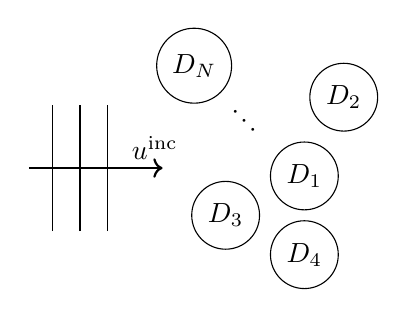
\begin{tikzpicture}
		\node[circle,draw] (c) at (0,0){$D_1$};
		\node[circle,draw] (c) at (0.5,1){$D_2$};
		\node[circle,draw] (c) at (-1,-0.5){$D_3$};
		\node[circle,draw] (c) at (0,-1){$D_4$};
		\node[circle,draw] (c) at (-1.4,1.4){$D_N$};
		\coordinate [label={[below,yshift=.1cm,rotate=135]$\dots$}](Dots2) at ({1*cos(150)},{1*sin(150)});
		
		% Draw the incoming wave (plane wave)
		\foreach \y in {0.1} {
			\draw[ thick, ->, domain=-3.5:-1.8, samples=50, smooth, variable=\x] plot (\x, \y );
		}
		
		\foreach \x in {-3.2, -2.85, -2.5}{
			\draw[ domain=-0.7:0.9, samples=50, smooth, variable=\y] plot (\x, \y );
		}
		
		\node at (-1.9, 0.35) {$u^\mathrm{inc}$};
	\end{tikzpicture}
\end{document}